\documentclass[pdflatex,sn-apa]{sn-jnl}

\usepackage{graphicx}%
\graphicspath{{figs/}}%
\usepackage{multirow}%
\usepackage{amsmath,amssymb,amsfonts}%
\usepackage{amsthm}%
\usepackage{mathrsfs}%
\usepackage[title]{appendix}%
\usepackage{xcolor}%
\usepackage{textcomp}%
\usepackage{manyfoot}%
\usepackage{booktabs}%
\usepackage{algorithm}%
\usepackage{algorithmicx}%
\usepackage{algpseudocode}%

\theoremstyle{thmstyleone}%
\newtheorem{theorem}{Theorem}%
\newtheorem{proposition}[theorem]{Proposition}%
\newtheorem{lemma}[theorem]{Lemma}%

\theoremstyle{thmstyletwo}%
\newtheorem{remark}{Remark}%

\theoremstyle{thmstylethree}%
\newtheorem{definition}{Definition}%
\newtheorem{assumption}{Assumption}%

\newcommand{\indep}{\perp\!\!\!\perp}
\newcommand{\Fcal}{\mathcal{F}}
\newcommand{\Scal}{\mathcal{S}}
\newcommand{\Gstar}{\mathcal{G}^{\star}}
\newcommand{\pa}{\mathrm{pa}}
\newcommand{\de}{\mathrm{de}}
\newcommand{\Prob}{\mathbb{P}}
\newcommand{\Exp}{\mathbb{E}}
\newcommand{\Real}{\mathbb{R}}

\raggedbottom

\begin{document}

\title[Transfer of causal discovery to real measurements]{Does causal discovery transfer to real measurements? A multi-dataset evaluation on cause--effect pairs, protein signalling and physical devices}

\author*[1]{\fnm{Quang-Vinh} \sur{Dang}}\email{vinh.dq4@buv.edu.vn}

\affil*[1]{\orgname{British University Vietnam}, \orgaddress{\city{Hung Yen}, \country{Vietnam}}}

\abstract{Causal discovery methods are usually validated on simulated data. We evaluate
fourteen methods on four families of real data with a known or consensus structure: the
Tübingen cause--effect pairs, the protein-signalling data of Sachs et al., and
two kinds of recordings from the Causal Chambers, physical devices with a known graph.
Besides established baselines (PC, GES, DirectLiNGAM, NOTEARS, IGCI, RECI, ANM-HSIC and a
pairwise LiNGAM rule), we include six methods we developed for this study and froze
before the evaluation: sequential certificates for edges and directions, PC with a
nonparametric test, a block-replicated additive method (BTAD), and two classifiers
trained on simulated data. The results are mixed and often unfavourable to the new
methods. On pairs, a regression-error rule (RECI) is the best or tied best method on
every real data set ($61\%$ on Tübingen, $94\%$ to $98\%$ on the chambers), and a
classifier that reaches $95\%$ on simulated pairs is at chance on Tübingen. On graphs,
DirectLiNGAM and GES are best on the chamber recordings with independent rows (skeleton
$F_1$ $0.55$ on the first two, $0.70$ on two others), while the methods using nonparametric tests are better on the
Sachs data ($F_1$ $0.62$ to $0.67$ against $0.52$ to $0.58$, with $17$ reference edges).
Seventeen of the nineteen new chamber recordings are random walks with an effective
sample size of a few observations out of $4000$, which makes tests that assume independent
rows reject roughly five times more graph-implied independences than a block test, and no
method exceeds $F_1=0.42$ there. We report where each method helps, where it does not,
and which of our design choices were fixed before and after seeing the data.}

\keywords{causal discovery, benchmark, real data, cause--effect pairs, Causal Chambers, serial dependence}

\pacs[MSC Classification]{62H22, 62G10, 68T05}

\maketitle


\section{Introduction}\label{sec:intro}

Methods for learning causal structure from observational data are mostly validated on
simulated data, where the generating mechanism is known and the assumptions of the method
can be matched to it. Real measurements differ in ways that simulation rarely reproduces:
mechanisms are nonlinear and heterogeneous, sensors are collinear, unobserved processes
induce dependence between measured variables, and rows are often not independent draws.
Benchmarks with real data and a known structure exist, but each covers a narrow slice:
the Tübingen cause--effect pairs \citep{mooij2016distinguishing}, the protein-signalling
data of \citet{sachs2005causal}, whose reference network is a contested consensus
\citep{mooij2020joint}, and, more recently, the Causal Chambers, physical devices whose
graph is known from their construction \citep{gamella2025chamber}.

This paper asks a plain question: when methods are applied unchanged to several real
data families, which ones work, and do recent ideas beat simple baselines? We evaluate
fourteen methods on four families of real data, under a protocol in which every method and
every setting was fixed and recorded before the data it is scored on were run, with the
exceptions listed in Section~\ref{sec:provenance}. The methods are eight established
baselines (PC, GES, DirectLiNGAM, NOTEARS for graphs; IGCI, RECI, ANM-HSIC and a pairwise
LiNGAM rule for pairs) and six methods that we developed during the project that produced
this study: sequential certificates for adjacency and direction, PC with a nonparametric
test, a block-replicated additive method, and two classifiers trained on simulated data.
Including our own methods is deliberate. Several were designed to address failures of the
baselines, and the comparison tells whether the design worked on measurements.

\paragraph{Contributions.}
\begin{enumerate}
\item A multi-dataset evaluation with a recorded protocol. It covers $102$ Tübingen
  pairs, $216$ pair analyses of edges of the Causal Chambers, the Sachs data, and
  $21$ chamber recordings with a known graph, and it reports a strict score against the
  reference graph and a score adjusted for dependences the graph cannot explain.
\item The result that, on pairs, a regression-error rule is the best or tied-best method on
  every real data set, and a classifier trained on simulated pairs, accurate on its
  simulated test set, is at chance on Tübingen (Section~\ref{sec:pairs}).
\item The result that, on graphs, the ranking of methods depends on the data family: DirectLiNGAM
  and GES on chamber recordings with independent rows, methods with nonparametric tests on the
  Sachs data, and no method on the random-walk recordings (Section~\ref{sec:graphs}).
\item A diagnosis of why the walk recordings defeat every method: their exogenous variables are
  random walks with an effective sample size of a few observations, so tests that assume
  independent rows reject graph-implied independences about five times more often than a block
  test, and a reference set built with them is contaminated (Section~\ref{sec:serial}).
\item The places where our own methods do help: control of false edges under repeated
  inspection and under nonlinear mechanisms in simulation (Section~\ref{sec:monitoring}).
\end{enumerate}

\paragraph{What the paper does not claim.} It does not claim that the methods we did not
evaluate (LOCI, QCCD, CAM, DAGMA, PCMCI+ and amortised methods such as AVICI
\citep{lorch2022amortized}) fail on these data, and it does not claim that the data
sets are representative of causal discovery in general. Several data sets have few
reference edges, so most differences between methods are within sampling error, and we
give intervals where we can.


\section{Data and protocol}\label{sec:data}

\subsection{Data}

\paragraph{Tübingen pairs.} The $102$ scalar-scalar pairs of the cause--effect benchmark
\citep{mooij2016distinguishing}, with the official weights. Tied values are dequantised by
adding uniform noise of the width of the smallest gap, long pairs are subsampled to $2000$
rows, and the preprocessing seed is fixed.

\paragraph{Causal Chambers.} The wind tunnel and the light tunnel \citep{gamella2025chamber}
are physical devices with a graph given by their construction. We use recorded experiments
in which the actuators vary, and the nodes of the chamber graph with at least $20$ distinct
values. Three kinds of recordings occur. In the \emph{i.i.d.} recordings the actuators are
redrawn independently at random: the wind tunnel with random intake loads and the light
tunnel with uniform inputs, used for the pair and graph evaluations (two recordings with
ten subsamples each). In the \emph{walk} recordings the actuators follow random walks:
$15$ runs of the wind tunnel, the pressure-control experiment, and three light-tunnel
experiments, of which one (\texttt{color\_mix}) is a walk and two have nearly independent rows
(Section~\ref{sec:serial}). The graphs have $8$ to $39$ edges among $10$ to $20$ variables
and are bipartite: settings point to measurements.

\paragraph{Sachs.} The $853$ observational cells with $11$ phosphoproteins, log-transformed;
the reference network is the $17$-arc consensus of \citet{sachs2005causal}, which is
contested \citep{mooij2020joint}.

\subsection{Scores}

\emph{Pairs.} Forced-choice accuracy of the direction (unweighted, and weighted by the
Tübingen weights), with Clopper--Pearson intervals; and accuracy at a given coverage when
pairs are ranked by a method's confidence.

\emph{Graphs.} Precision, recall and $F_1$ of the skeleton against the reference graph
(``strict''). Because the chamber graphs do not explain all dependence among the sensors
(for instance four barometers share an ambient pressure), we also report precision against
the graph plus a reference set $V$ of non-adjacent pairs whose graph-implied conditional
independence is rejected on held-out rows (``adjusted''); the strict score is the headline.

\subsection{Effective sample size}\label{sec:ess}

For each recording we measure the lag-1 autocorrelation $\rho$ of the exogenous
variables and the implied effective sample size $n(1-\rho)/(1+\rho)$ of the first $4000$ rows.
The result (Section~\ref{sec:serial}) splits the nineteen new recordings into two with an
effective sample size above $1000$ and seventeen below $20$.

\subsection{Protocol and provenance}\label{sec:provenance}

Methods, settings and the scripts that score them were committed to the repository
before the run in every case except the following, which are post hoc and flagged where they
occur. First, the Causal Chambers recordings with independent rows and the Sachs data were
inspected while we were developing the sequential certificates, so those certificates
were adjusted after seeing them (a nonparametric test, a larger conditioning order). Second,
the nine simulated pair families used to choose the agreement rule of the direction
certificate are design data. Third, the reference set $V$ was introduced after seeing
false edges. Every other number is from a frozen run: the new chamber recordings, the
Tübingen pairs for all methods, the learned models (trained only on simulated data and
frozen before evaluation), the baselines, and the Sachs run of all methods. The six
methods of the study and their settings are described in Section~\ref{sec:methods} and the
appendix.


\section{Methods compared}\label{sec:methods}

\subsection{Established baselines}

\emph{Graphs.} PC with Fisher-$z$ tests at $\alpha=0.05$ and $0.01$ \citep{spirtes2000causation},
GES with the BIC score \citep{chickering2002optimal}, DirectLiNGAM
\citep{shimizu2011directlingam} with edges thresholded at $|B|>0.05$, all from
\texttt{causal-learn}; NOTEARS with a linear model \citep{zheng2018dags} (our compact
re-implementation, $\ell_1$ penalty $0.1$, threshold $0.3$); DAGMA, linear with the $\ell_2$ loss
(package \texttt{dagma}, $\lambda_1=0.03$, threshold $0.3$); and PCMCI+ \citep{runge2020discovering} from
\texttt{tigramite} with partial-correlation tests, lags $0$ and $1$, $\alpha=0.01$, taking the
contemporaneous links as the skeleton. We score skeletons only.

\emph{Pairs.} IGCI in its entropy form with a uniform reference \citep{daniusis2010inferring},
RECI, which prefers the direction with the smaller regression error after min--max scaling
\citep{blobaum2018cause}, an additive noise model with a spline regression and an HSIC
independence criterion (ANM-HSIC; \citealt{hoyer2009nonlinear}), and the first-order pairwise
LiNGAM likelihood-ratio statistic \citep{hyvarinen2013pairwise}. These are short
re-implementations of the published rules and were not tuned. We add a Gaussian-process additive
noise model (\texttt{causal-learn}, direction with the larger independence $p$-value, $400$ rows)
and LOCI \citep{immer2023loci}, run with the authors' public code in its default setting (neural
network, $5000$ steps, HSIC independence test, at most $1000$ rows per pair).

\subsection{Methods developed for this study}

All six were frozen before their evaluation on the data in which they are scored, except
where Section~\ref{sec:provenance} says otherwise. Details are in the appendix.

\paragraph{Direction certificate (relative fit).} For a pair, two forecasters of the joint
law, one per factorisation, are fitted sequentially on past rows; the running mean of the
log-score difference has an asymptotic confidence sequence
\citep{waudbysmith2024asymptotic}; a direction is reported only when two model classes
(constant scale and location-scale generalised Gaussian) agree. It abstains on most pairs.
It certifies better predictive fit, not causation.

\paragraph{CERT-CD (sequential adjacency certificates).} An edge is asserted only when,
for every conditioning set of size at most $k$, a sequential test of conditional dependence
has rejected. We use the nonparametric version, a sequential generalised covariance test
\citep{shah2020hardness} with spline regressions, at $k=3$ on the chambers.

\paragraph{PC with a nonparametric test (PC-GCM).} PC (depth at most $3$) with the same
test used as PC uses a test: cross-fitted residuals, three residual products, an edge is
deleted when some conditioning set yields a $p$-value above $\alpha$. It separates the effect of the
test from the effect of the sequential architecture.

\paragraph{BTAD (block-replicated additive discovery).} Time-ordered rows are cut into
$60$ contiguous blocks. A variable is added to a node's Markov blanket when its held-out
gain in an additive spline model replicates across blocks (one-sided $t$ test, Bonferroni
over candidates), blankets are grown and shrunk, and edges that a small subset of the union
of two blankets can explain away are removed. Its settings were fixed on simulated data
($\alpha=0.2$, blanket at most $8$).

\paragraph{LRG (learned replicated-gain model).} A gradient-boosting classifier on $25$
features per pair (block gains with several conditioning sets, correlation,
autocorrelation, within-data-set ranks), trained on $600$ simulated data sets with
nonlinear mechanisms, serial dependence, latent drift and duplicated sensors. The decision
threshold is set on a validation split of the simulations.

\paragraph{PDM (pair-direction model).} A gradient-boosting classifier on $32$ features
(spline regression errors at three flexibilities, residual dependence, residual shape,
IGCI entropies, Gaussian and location-scale log-likelihoods, the pairwise LiNGAM
statistic, discreteness) trained on $40000$ simulated pairs with $12$ mechanism families,
$6$ noise laws, additive, multiplicative, location-scale and post-nonlinear structure,
quantisation and serial dependence. This is the learned approach of
\citet{lopezpaz2015towards} with different features and simulator.


\section{Results}\label{sec:results}

\subsection{Cause--effect pairs}\label{sec:pairs}

Figure~\ref{fig:pairs} and Table~\ref{tab:pairs} give the forced-choice accuracy of the
learned model PDM, LOCI, a Gaussian-process ANM and the four rules on the pair sets. RECI has
the highest accuracy on both chamber sets: $97.9\%$ on the i.i.d.\ pairs and $94.3\%$ on the pairs of
the further recordings. The differences from IGCI ($93.6\%$, $88.5\%$; exact McNemar $p=0.29$ and
$0.17$) are not significant, nor is the difference from PDM on the i.i.d.\ pairs ($p=0.18$); RECI is
significantly more accurate than LOCI ($76.6\%$, $68.0\%$), the Gaussian-process ANM, ANM-HSIC and the
pairwise LiNGAM rule ($p<0.001$ in both sets). On Tübingen LOCI has the highest unweighted accuracy ($64.7\%$, interval
$[54.6,73.9]$, weighted $63.9\%$) and RECI, ANM-HSIC and the LiNGAM rule have $60.8\%$
($[50.6,70.3]$; RECI weighted $70.9\%$, the highest weighted accuracy, with LOCI third). None of these
differences is significant (exact McNemar $p\ge0.23$ for RECI against every other method except PDM).
Our LOCI run uses at most $1000$ rows per pair and the authors' default settings, and its accuracy
may be below published values (Section~\ref{sec:loci-check}). The
Gaussian-process ANM has $55.4\%$ when its $23$ exact ties (a score of zero) are counted as half correct. On the $17$ Sachs pairs (which share $11$ variables) every method lies between $47\%$ and
$65\%$ and every interval contains $50\%$ and is about $50$ points wide. PDM, which reaches $95\%$ on its
held-out simulated test set and $83\%$ on nine unseen simulated families, has $40.2\%$ on Tübingen
(interval $[30.6,50.4]$, exact binomial $p=0.059$ against $50\%$), significantly below RECI (McNemar
$p=0.002$), and is below RECI and IGCI on both chamber sets. The only pair set on which it is
best is the simulated one, which is its own prior.

\begin{figure}[t]
\centering
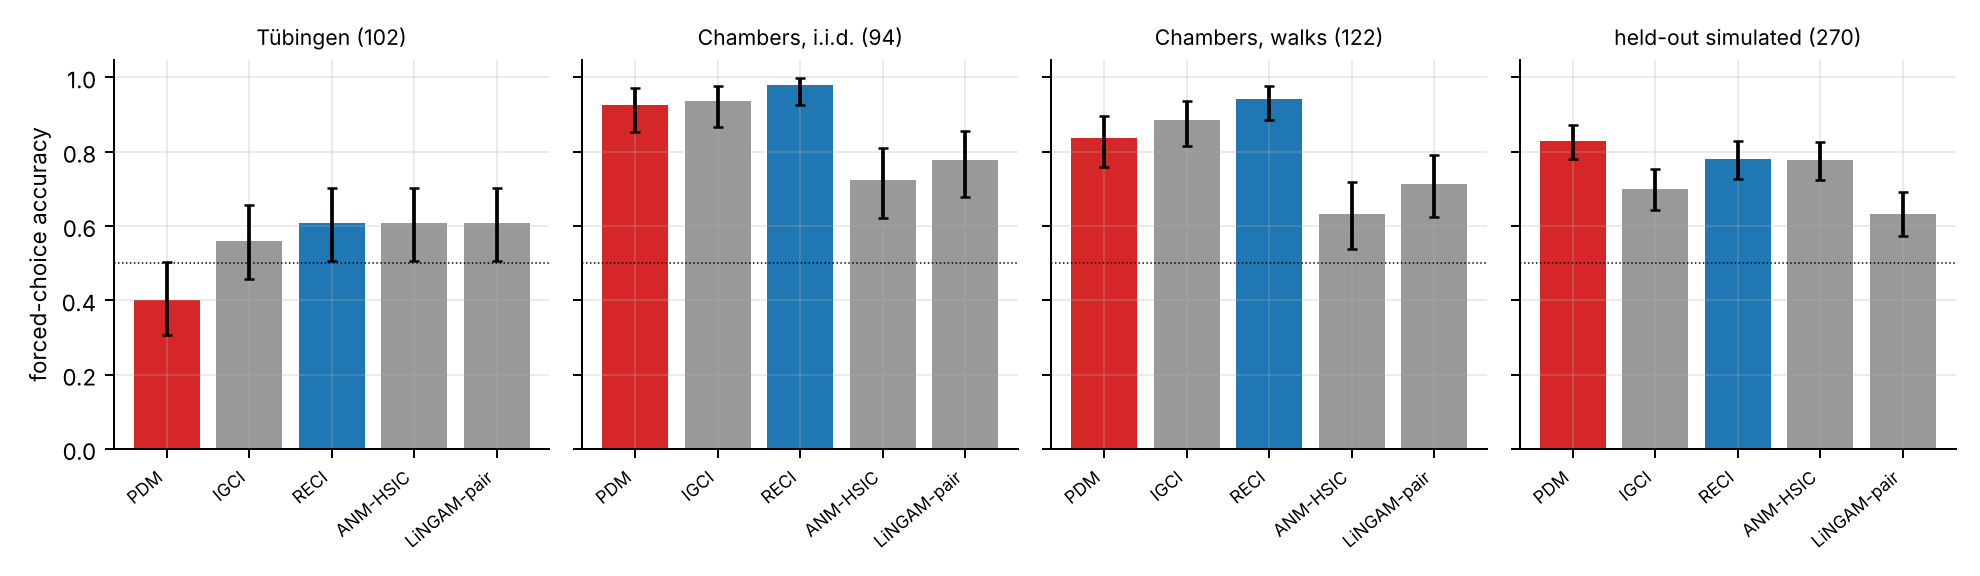
\includegraphics[width=\linewidth]{pairs_accuracy.png}
\caption{Forced-choice accuracy with Clopper--Pearson intervals on five pair sets (pairs or
pair-runs in parentheses). Red: PDM; green: LOCI; blue: RECI; grey: the other rules. Dotted:
chance. LOCI and the Gaussian-process ANM were not run on the simulated families.}
\label{fig:pairs}
\end{figure}

\begin{table}[t]
\caption{Forced-choice accuracy (unweighted; weighted by the official weights for Tübingen).
LOCI and ANM were not run on the simulated families. $^{\dagger}$Exact ties (a score of zero; $23$
pairs) are counted as half correct.}
\label{tab:pairs}
\small
\setlength{\tabcolsep}{2.5pt}
\begin{tabular}{@{}lccccc@{}}
\toprule
Method & Tübingen & chambers iid & chambers, further & Sachs & simulated\\
 & ($102$) & ($94$) & ($122$) & ($17$) & ($270$)\\
\midrule
PDM & 0.402 (0.511) & 0.926 & 0.836 & 0.529 & 0.830\\
LOCI & 0.647 (0.639) & 0.766 & 0.680 & 0.471 & --\\
ANM, Gaussian process$^{\dagger}$ & 0.554 (0.594) & 0.771 & 0.672 & 0.559 & --\\
IGCI & 0.559 (0.664) & 0.936 & 0.885 & 0.647 & 0.700\\
RECI & 0.608 (0.709) & 0.979 & 0.943 & 0.529 & 0.781\\
ANM-HSIC & 0.608 (0.609) & 0.723 & 0.631 & 0.588 & 0.778\\
pairwise LiNGAM & 0.608 (0.620) & 0.777 & 0.713 & 0.529 & 0.633\\
\bottomrule
\end{tabular}
\end{table}

\paragraph{LOCI with more rows.}\label{sec:loci-check} Raising the row cap from $1000$ to $2000$ (the preprocessing of the other
methods) gives $65.7\%$ on Tübingen (interval $[55.6,74.8]$, weighted $66.4\%$) and $97\%$ of the directions agree
with the $1000$-row run, so the cap does not explain the accuracy. We did not reproduce a higher published value
and cannot rule out that the settings or the preprocessing differ from the authors'.

\paragraph{Abstention.} The direction certificate commits on $12$ of the $80$ scorable
Tübingen pairs and is right on $11$. Ranked by its own confidence, RECI is right on $11$ of
its $12$ most confident pairs, and on $21$ of $23$ against $19$ of $23$ at the coverage of the
constant-scale class. On the chamber pairs the certificate is right on all $31$ pairs it
commits to ($94$ pair-runs), as are the RECI and IGCI rankings at that coverage; on the
simulated pairs it is right on $78$ of $83$ against $82$ of $83$ for RECI. At matched coverage the
certificate is therefore not more accurate than RECI; what it adds is that it chooses its
own coverage from the data. The Tübingen result of the certificate is stable over random
draws of the preprocessing ($9/9$, $11/11$, $10/10$ for three further seeds), and its one
error occurred on a pair with $254$ rows.

\subsection{Graphs}\label{sec:graphs}

Table~\ref{tab:graphs} and Figure~\ref{fig:graphs} give the skeleton score on the graph
benchmarks. The ranking of methods depends on the data family.

\begin{table}[t]
\caption{Skeleton precision / recall / $F_1$ against the reference graph (strict); mean over
recordings or subsamples. Sachs: one data set, $17$ reference edges. Chambers i.i.d.: two
recordings, ten subsamples of $4000$ rows each. Chambers with an effective sample size above
$1000$ (two recordings) and below $20$ (seventeen recordings): the first $4000$ rows in time
order. Best $F_1$ in bold.}
\label{tab:graphs}
\scriptsize
\setlength{\tabcolsep}{2pt}
\begin{tabular}{@{}lcccc@{}}
\toprule
Method & Sachs & Chambers iid & ESS $>1000$ & ESS $<20$\\
\midrule
PC, $\alpha=0.05$ & 1.00/0.41/0.58 & 0.40/0.38/0.37 & 0.48/0.28/0.35 & 0.36/0.39/0.37\\
GES-BIC & 1.00/0.41/0.58 & 0.45/0.64/0.49 & 0.74/0.67/\textbf{0.70} & 0.26/0.71/0.38\\
DirectLiNGAM & 1.00/0.35/0.52 & 0.55/0.60/\textbf{0.55} & 0.71/0.63/0.66 & 0.26/0.63/0.37\\
NOTEARS & 1.00/0.18/0.30 & 0.41/0.21/0.27 & 0.33/0.24/0.26 & 0.26/0.45/0.33\\
DAGMA & 1.00/0.29/0.45 & 0.44/0.33/0.36 & 0.44/0.41/0.39 & 0.25/0.52/0.34\\
PCMCI+ & 1.00/0.35/0.52 & 0.39/0.33/0.34 & 0.53/0.29/0.37 & 0.27/0.17/0.20\\
PC, nonparam.\ test & 0.89/0.47/0.62 & 0.38/0.33/0.34 & 0.54/0.34/0.41 & 0.35/0.54/\textbf{0.42}\\
BTAD & 0.89/0.47/0.62 & 0.56/0.36/0.41 & 0.82/0.46/0.58 & 0.60/0.16/0.25\\
LRG & 0.90/0.53/\textbf{0.67} & 0.39/0.48/0.43 & 0.52/0.55/0.53 & 0.51/0.28/0.36\\
CERT-CD, nonparametric & 1.00/0.29/0.45 & 0.29/0.16/0.20 & 0.60/0.18/0.28 & 0.24/0.87/0.37\\
\bottomrule
\end{tabular}
\end{table}

\begin{figure}[t]
\centering
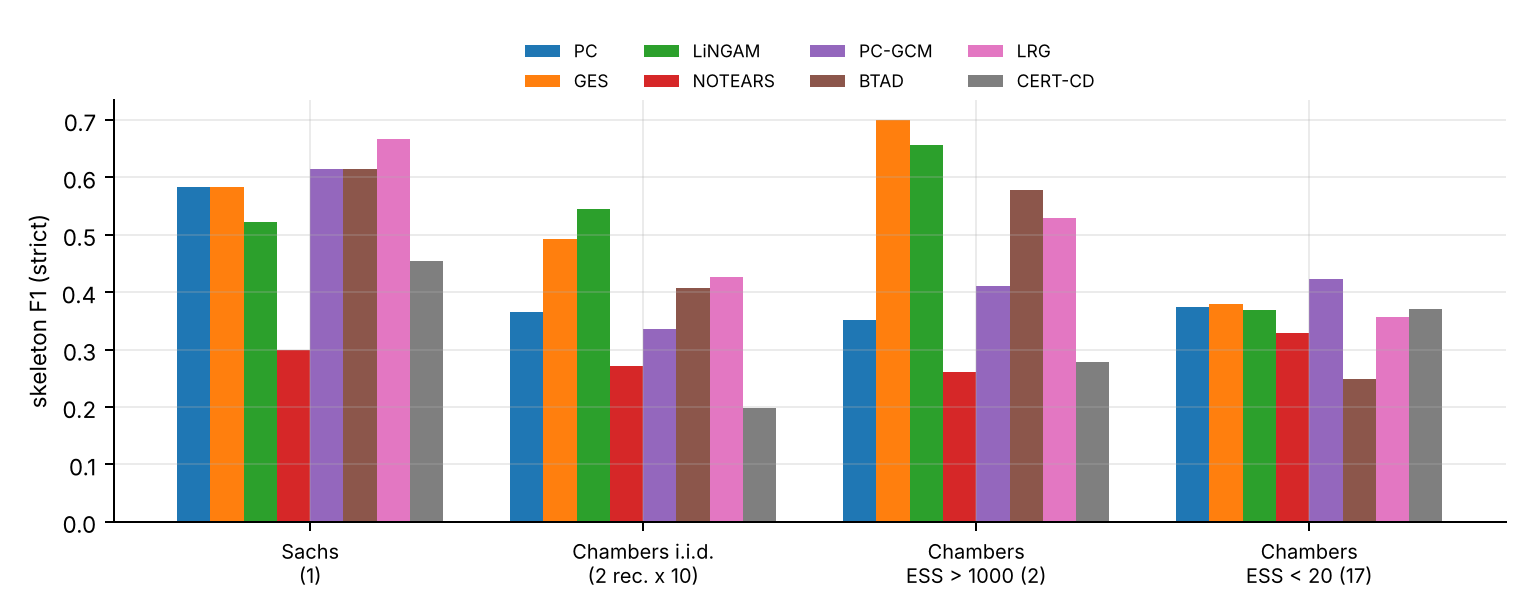
\includegraphics[width=0.95\linewidth]{graph_f1.png}
\caption{Strict skeleton $F_1$ by data family and method.}
\label{fig:graphs}
\end{figure}

\paragraph{Sachs.} The methods we developed that use nonparametric components have the
highest $F_1$ (LRG $0.67$, PC with the nonparametric test $0.62$--$0.64$, BTAD $0.62$), against $0.58$
for PC and GES, $0.52$ for DirectLiNGAM and PCMCI+, $0.45$ for DAGMA and $0.30$ for the linear NOTEARS. The reference network
has $17$ edges, so one edge changes recall by $0.06$ and the differences are not statistically
distinguishable; the classical methods have the highest precision ($1.00$) and the new ones
find a few more edges.

\paragraph{Chambers with independent rows.} DirectLiNGAM and GES have the highest $F_1$. On the two
recordings with i.i.d.\ actuators DirectLiNGAM has $F_1=0.55$ and GES $0.49$, against
$0.32$ to $0.43$ for PC with either test, BTAD and LRG; on the two further recordings with
a large effective sample size GES has $0.70$ and DirectLiNGAM $0.66$. The actuators there
are uniform and the mechanisms may be nearly additive, which would suit DirectLiNGAM (we did not test
this explanation); each group has two recordings and no interval can be given. BTAD has the highest
precision ($0.56$, against $0.55$ for DirectLiNGAM, and $0.82$) at lower recall. The sequential
certificate has the lowest $F_1$ on the i.i.d.\ recordings ($0.20$).

\paragraph{Random-walk recordings.} On the seventeen recordings with an effective sample size
below $20$ every method has a strict $F_1$ between $0.20$ and $0.42$; the best, PC with the nonparametric test,
has precision $0.35$. BTAD has the highest precision ($0.60$, with $2.5$ false edges per
recording against $16$ to $52$ for PC, GES and DirectLiNGAM) and recall $0.16$. PCMCI+, the method
built for autocorrelated series, has recall $0.17$ and $F_1=0.20$ there, as expected when the
recordings contain no usable lag structure (Section~\ref{sec:serial}); DAGMA has $F_1=0.34$. Paired Wilcoxon tests over the $15$
wind-tunnel recordings, with Holm correction over the eleven comparisons, show that BTAD's $F_1$ is
lower than that of ten of the other methods (adjusted $p\le0.02$) and higher than that of PCMCI+; LRG is not
distinguishable from PC, GES or DirectLiNGAM.

\subsection{The walk recordings carry a few independent observations}\label{sec:serial}

Figure~\ref{fig:serial} shows why the walk recordings defeat every method. In the fifteen
wind-tunnel walks the mean lag-1 autocorrelation of the exogenous variables is $0.998$ and
the implied effective sample size is about $3$ of $4000$ rows (range $1.3$ to $12.5$). The mean
cross-correlation between a load and the rotation speed it drives varies by only $0.012$ for lags from $-6$
to $+6$ ($0.974$ to $0.985$), so the recordings also contain no usable lag structure. An i.i.d.\ test
of the independences implied by the graph rejects $40.8$ non-adjacent pairs per recording on the wind-tunnel
walks and a test on $40$ contiguous blocks rejects $8.5$, a ratio of $4.8$; over the seventeen recordings with an
effective sample size below $20$ the ratio is $4.1$ ($38.9$ against $9.5$), over all nineteen $3.7$, for
the pressure-control recording $2$ and for the light-tunnel walk $1$ ($21$ against $21$). The block
test has lower power by construction, so a smaller number of rejections does not by itself show that the
i.i.d.\ rejections are artefacts; it does show that a reference set built with the i.i.d.\ test has
many more pairs than one built with a test that respects serial dependence, and that scores adjusted
for it should be read with caution. Two
recordings of the new set (\texttt{actuators\_white}, \texttt{smooth\_polarizers}) have an
effective sample size above $1000$, and on these two the classical methods have the highest $F_1$; two
recordings are too few to separate effective sample size from device. We did not run a controlled test
(thinning, or a time-series-aware test on the same recordings), which would be the direct evidence.

\begin{figure}[t]
\centering
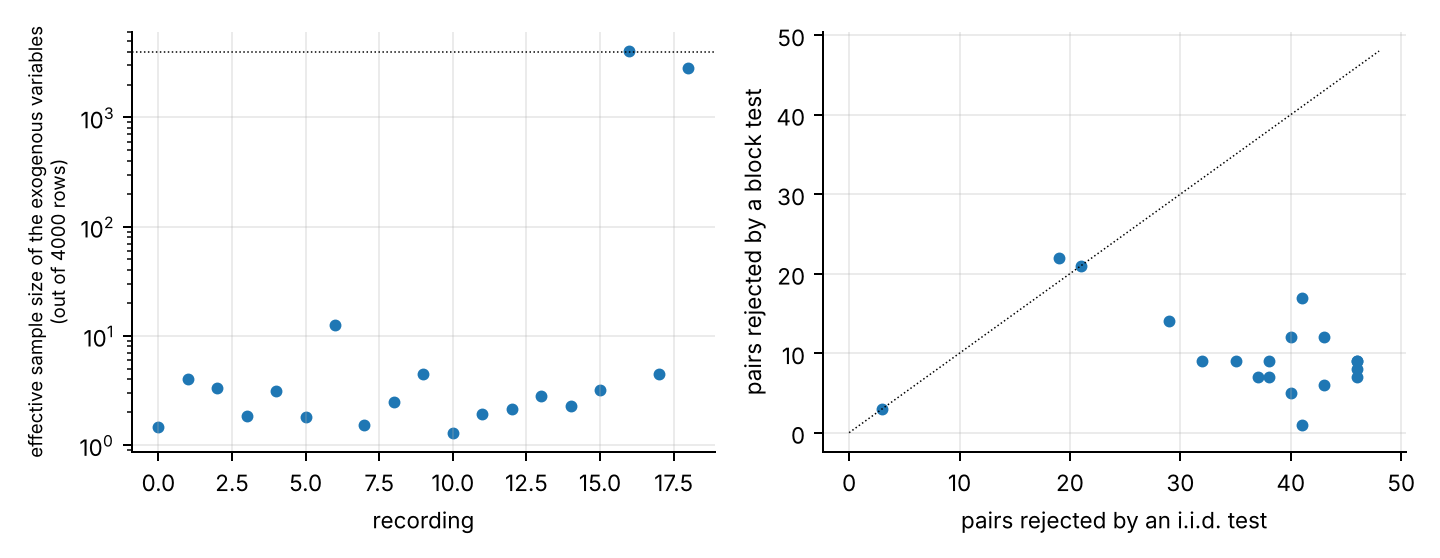
\includegraphics[width=0.9\linewidth]{serial_dependence.png}
\caption{Left: effective sample size (log scale) of the exogenous variables in each of the
nineteen new recordings. Right: number of non-adjacent pairs whose graph-implied independence
is rejected by an i.i.d.\ test and by a block test.}
\label{fig:serial}
\end{figure}

\subsection{Where the new methods help: monitoring and nonlinear mechanisms}\label{sec:monitoring}

On simulated graphs the sequential certificate does what it was designed for
(Table~\ref{tab:monitoring}). When each method is rerun at every sample size from $100$ to
$6400$ on $150$ random eight-node graphs and a graph counts as a failure if any estimate
contains a false edge, CERT-CD fails in $2.7\%$ of the graphs under Laplace errors, against
$27\%$ to $91\%$ for PC, GES and DirectLiNGAM and $39\%$ to $77\%$ for PC with the same
nonparametric test, which is consistent with the delete-on-non-rejection architecture, and not the test, being responsible
(a single comparison). With nonlinear mechanisms the linear test of the certificate fails in $33$
of $60$ graphs under Laplace errors and $28$ of $60$ under Gaussian errors, and the nonparametric
version in $1$ and $2$ of $60$. The guarantee of the linear version is exact only for
Gaussian regression errors, and that of the nonparametric version is asymptotic. The table shows false
edges only, not power: the recall of the nonparametric certificate is $0.00$ at $n=100$ and $0.05$ at
$n=200$ under Laplace errors, and DirectLiNGAM is run on Gaussian errors, which violate its assumption.
These are simulations within the models; on the chambers the false-edge control did not hold
(a false edge adjusted for a reference set built with an i.i.d.\ test in $12$ of $19$ recordings, a strict false edge in $18$, with shuffled rows).

\begin{table}[t]
\caption{Probability that a false edge is ever reported over $n=100,\dots,6400$ ($150$ graphs,
$d=8$), and graphs with a false edge under nonlinear mechanisms ($60$ graphs).}
\label{tab:monitoring}
\small
\begin{tabular}{@{}lcc@{}}
\toprule
Method & Laplace errors & Gaussian errors\\
\midrule
CERT-CD, linear test & 0.027 & 0.040\\
CERT-CD, nonparametric test & 0.060 & 0.047\\
PC, $\alpha=0.05$ / $0.01$ & 0.747 / 0.267 & 0.773 / 0.320\\
PC, nonparametric test, $\alpha=0.05$ / $0.01$ & 0.767 / 0.387 & 0.787 / 0.320\\
GES-BIC & 0.913 & 0.960\\
DirectLiNGAM & 0.760 & 1.000\\
\midrule
nonlinear mechanisms: linear test (of $60$) & 33 & 28\\
nonlinear mechanisms: nonparametric test (of $60$) & 1 & 2\\
\bottomrule
\end{tabular}
\end{table}

\subsection{The gap between simulation and measurement}\label{sec:gap}

The two learned models are accurate on data from their training distribution and lose that
on real data (Table~\ref{tab:gap}). PDM falls from $0.95$ to $0.40$ on Tübingen; LRG falls
from an $F_1$ of $0.86$ on simulated graphs to $0.36$--$0.43$ on the chambers, and its
within-recording ranking of pairs on the wind-tunnel walks is close to chance (mean AUC $0.55$ over $15$
recordings, range $0.51$ to $0.60$).
We cannot say which feature of the real data is responsible; the simulators contain serial
dependence, latent drift, duplicated sensors and several mechanism families and still do not
cover them.

\begin{table}[t]
\caption{Learned models: simulated test against real data.}
\label{tab:gap}
\small
\begin{tabular}{@{}lccc@{}}
\toprule
Model & simulated test & real data & measure\\
\midrule
PDM & 0.95 / 0.83 & 0.40 Tübingen; 0.93, 0.84 chambers & forced accuracy\\
LRG & 0.86 & 0.67 Sachs; 0.43, 0.53, 0.36 chambers & skeleton $F_1$\\
\bottomrule
\end{tabular}
\end{table}


\section{Discussion}\label{sec:discussion}

\paragraph{What the evidence supports.} On the real data we examined, simple methods are hard
to beat. On pairs the best method on the chambers is RECI, which compares two regression errors, and on
Tübingen no method is distinguishable from RECI, with LOCI nominally ahead; on graphs the
best methods on recordings with independent rows are DirectLiNGAM and GES, and on the Sachs
data a mix of methods that use nonparametric tests, with differences smaller than the sampling
error of a $17$-edge reference. The methods we developed to address specific failures show their
intended benefit in simulation and some of it on measurements: lower false-edge rates under
repeated inspection and nonlinear mechanisms in simulation, and the highest precision on the
chamber recordings, BTAD, at the price of recall. None of them has the best $F_1$ on the
chambers. The two classifiers trained on simulated data are the clearest negative results, and
we think they are informative: a model that is nearly perfect on a broad simulator can be at
chance on real pairs.

\paragraph{Implications for evaluation.} First, the effective sample size of a recording
should be reported: seventeen of nineteen new chamber recordings had fewer than twenty
effective observations, which no test that assumes independent rows can cope with, and which
also contaminates reference sets built with such tests. Second, adjusting the score for
dependences the reference graph cannot explain changes conclusions and should be shown next to the
strict score, with the construction of the adjustment disclosed and made independent of the methods.
Third, the protocol matters: several of our early positive results were produced by
choices made after seeing the data, and the frozen evaluation reversed them. We report which
numbers are frozen and which are not (Section~\ref{sec:provenance}).

\paragraph{Limitations.} The reference networks are small, the Sachs consensus is contested,
and the chamber graphs are bipartite, so recovery of the skeleton is mostly feature selection
from actuators to measurements. Most differences between graph methods are within sampling
error, and the effective sample size of the walk recordings limits what any method can show.
We did not evaluate amortised methods (AVICI), CAM or QCCD, and several baselines
are re-implementations or default runs (LOCI on at most $1000$ rows); a better-tuned baseline could change a ranking.
The Causal Chambers also contain interventional experiments, where a simple shift test already
recovers the descendants with perfect precision, and we did not use them. The new methods were
developed by the author of this paper, which is a source of bias; the frozen protocol and the
public code are the mitigation.


\backmatter


\bmhead{Competing interests} The author declares no competing interests.

\bmhead{Funding} This research received no specific grant from any funding
agency in the public, commercial, or not-for-profit sectors.

\bmhead{Ethics approval} Not applicable. The study involves no human
participants or animals. The protein-signalling data analysed in
Section~\ref{sec:data} are publicly available and were published by
\citet{sachs2005causal}.

\bmhead{Data and code availability} All simulation code, experiment scripts,
random seeds and figure-generating scripts are available at
\url{https://github.com/vinhqdang/SPRINT-CD}. The protein-signalling data of
\citet{sachs2005causal} are redistributed with the \texttt{bnlearn} package
\citep{scutari2010learning} and are downloaded by the experiment script rather
than included in the repository. The Tübingen cause-effect pairs of
Section~\ref{sec:data} are downloaded on first use from
\url{https://webdav.tuebingen.mpg.de/cause-effect/} and are not redistributed.

\bmhead{Author contributions} The author is solely responsible for all aspects
of this work.

\bmhead{Use of generative AI} A large language model was used in support of
writing this manuscript. The author verified and modified the resulting
content and takes full responsibility for the manuscript in its entirety,
including its claims, derivations, experiments and references.


\begin{appendices}

\section{Method details}\label{app:methods}

\paragraph{Pair features.} The direction hypothesis $c\to e$ is described by the log
cross-validated mean squared error of additive cubic spline regressions of $e$ on $c$ with
$2$, $4$ and $8$ knots, the log HSIC between the residual and the cause, the share of
$\log r^2$ explained by $c$, the skewness and kurtosis of the residual, the correlation of
$r^2$ with $c^2$, held-out Gaussian and location-scale log-likelihoods, and the spacing
entropy, skewness and kurtosis of $c$; the feature vector is the difference between the two
directions plus their sum and symmetric nuisance features (sample size, correlation, share of
distinct values). The classifier has depth $6$, $500$ trees and learning rate $0.05$.

\paragraph{Graph features (LRG).} For every pair, the held-out gain of adding one variable to
a model of the other with $40$ contiguous blocks (mean, $t$ statistic, share of positive
blocks), in both directions, with an empty conditioning set, the three strongest other
predictors, and the single conditioner that most explains the pair away; the absolute
correlation; the smaller and larger lag-1 autocorrelation of the two variables; the log
number of variables; and within-data-set ranks of the three $t$ statistics. Depth $4$, $300$
trees. The decision threshold ($0.4$) maximises validation $F_1$.

\paragraph{BTAD.} Spline ridge models with three knots at the quartiles, inputs clipped at
the $1\%$ and $99\%$ quantiles, pairwise products when the conditioning set has two or more
members; gap of $5\%$ of the block length between blocks; $60$ blocks; Bonferroni over the
candidates of each step; blanket of at most $8$ variables; spouse removal over subsets of
size at most $2$ of the union of the blankets.

\paragraph{PC with a nonparametric test.} Residuals of $X_v$ and $X_v^2$ on an additive spline
of $X_S$ with two-fold cross-fitting; the three products $r_ir_j$, $r_ir_j^{(2)}$ and
$r_jr_i^{(2)}$; $p$-value $=\min(1,3\min_k p_k)$.

\paragraph{Sequential certificates.} The adjacency certificate and the direction certificate
are described, with their assumptions, in the companion paper (\texttt{paper/certcd2} in the
repository); here only their outputs are used.

\paragraph{Reproduction.} Each experiment is a script in \texttt{experiments/}, committed
before it was run, with a summary script in \texttt{scripts/}; the figures are made by
\texttt{scripts/make\_benchmark\_figs.py}. All results are in \texttt{results/} as JSON.
Seeds are fixed. The Chamber data and the Tübingen pairs are downloaded on first use.

\end{appendices}

\bibliography{refs}

\end{document}
